% English version of paper/ja_v4/03_方法.md (ver4, 2026-11-17). The table of compared methods was removed at the researcher's request; the methods are listed in the text. Conditions are called by name (the code list (A0)--(E2) is Table S7). All procedure-order disclosures are gathered in Sect. 3.7 (Mensh & Kording rule 3). Sentences are carried over from v3_03_setup, v3_04_analysis (4.1, 4.2, 4.4), v3_05_method and v3_06_experiments where the Japanese text was carried over.
\FloatBarrier
\section{Methods}\label{sec:methods}

\subsection{Corpora and settings}\label{sec:setup}
We use six corpora that differ in elicitation, recording and annotation as seven groups (Table~\ref{tab:corpora}). IEMOCAP \cite{busso2008iemocap} is split into improvised and scripted groups, because in scripted sessions ten actors read the same lines and a text classifier could succeed by memorising them. Labels are mapped to the four emotions present in all seven groups, Neutral, Happy, Sad and Angry (the four emotions of Ryumina et al.\ \cite{ryumina2025}), and utterances with other labels are not used. IEMOCAP uses the plurality label of the raters, with neutral as Neutral, happy and excited as Happy, sad as Sad and angry as Angry; frustration is not mapped to Angry, and disgust, fear, surprise, other and utterances without a plurality are not used. MELD uses neutral, joy, sadness and anger, and AFEW and CREMA-D the labels corresponding to Neutral, Happy, Sad and Angry; disgust, fear and surprise are not used (CREMA-D has no surprise). RAVDESS uses neutral, happy, sad and angry; calm is not merged into Neutral, and calm, fearful, disgust and surprised are not used. In MOSEI, an utterance with exactly one emotion of intensity at least 0.5 receives that emotion, one with none receives Neutral, and one with two or more is not used, so MOSEI Neutral is not a neutral rating by annotators.

\begin{table}[t]
\caption{The seven groups. Elicitation, recording and annotation follow the original papers. Speaker and utterance counts are after restricting to four emotions, for the all-source setting (and the single-source setting of Supplementary Information S2); utterance and per-emotion counts are for the audio (WavLM) set, with differing visual or text counts in parentheses. The last column gives, for the LOCO setting (utterances with audio, visual and text; CREMA-D: audio and visual), the utterances, the clusters used to form test folds and their effective number $(\sum_g n_g)^2/\sum_g n_g^2$ for cluster sizes $n_g$; per-emotion LOCO counts are in Table~S1. Mod.: modalities. All corpora are in English (RAVDESS: North American English)}\label{tab:corpora}
\footnotesize\setlength{\tabcolsep}{3pt}
\begin{tabular}{@{}p{1.55cm}p{1.7cm}p{1.95cm}p{0.75cm}r p{1.5cm}p{1.7cm}p{1.35cm}@{}}
\toprule
Group & Elicitation, recording & Annotation & Mod. & Speakers & Utterances & N / H / S / A & LOCO (clusters, effective) \\
\midrule
AFEW \cite{dhall2012afew,dhall2013emotiw} & Movie acting (partly natural); scenes found by subtitle emotion words & Facial-expression category by raters & A, V, T$^{b}$ & 282$^{a}$ & 795 & 207 / 213 / 178 / 197 & 790 (51, 14.99) \\
IEMOCAP impro.\ \cite{busso2008iemocap} & Improvised acting; dyadic lab sessions & Plurality of raters' categories & A, V, T & 10 & 2,943 & 1,099 / 947 / 608 / 289 & 2,943 (5, 4.91) \\
IEMOCAP script.\ \cite{busso2008iemocap} & Scripted acting & Same & A, V, T & 10 & 2,588 (V 2,549) & 609 / 689 / 476 / 814 & -- \\
MOSEI \cite{zadeh2018mosei} & None (opinion monologues); YouTube videos & Crowd intensities of six emotions; our rule & A, V, T & 2,626$^{c}$ & 18,919 (V 18,634) & 8,847 / 6,790 / 1,830 / 1,452 & 18,634 (2,614, 783.22) \\
MELD \cite{poria2019meld} & TV-series acting; Friends multi-party scenes & Majority of raters' categories & A, V, T & 283 & 11,343 (V 11,308, T 11,344) & 6,430 / 2,305 / 1,002 / 1,606 & 11,267 (272, 8.59) \\
CREMA-D \cite{cao2014cremad} & Instructed acting, 12 sentences & Acted emotion; crowd ratings & A, V & 91 & 4,900 (V 4,899) & 1,087 / 1,271 / 1,271 / 1,271 & 4,899 (91, 90.98) \\
RAVDESS \cite{livingstone2018ravdess} & Instructed acting, 2 sentences & Acted emotion; validated by raters & A & 24 & 672 & 96 / 192 / 192 / 192 & -- \\
\botrule
\end{tabular}
\footnotetext{$^{a}$Number of actor names. $^{b}$AFEW text features come from Whisper large-v3 transcripts (790 utterances) and were made after the single-source and all-source computations, which therefore do not use them. $^{c}$Number of channels or video IDs (Sect.~\ref{sec:split}). The two IEMOCAP groups share the same ten actors. Concatenated features are built only from utterances that have all of the concatenated modalities. LOCO clusters: actor/movie links (AFEW), sessions (IEMOCAP), channels or videos (MOSEI), speakers (MELD, CREMA-D)}
\end{table}

The results in the main text were computed in two settings (Fig.~S1 of the Supplementary Information, Online Resource 1).
\begin{itemize}
\item \textbf{Leave-one-corpus-out (LOCO) setting} (Sects.~\ref{sec:res-methods} and \ref{sec:res-margin}--\ref{sec:res-retrain}): one of AFEW, IEMOCAP (improvised part only), MOSEI and MELD, which have audio, visual and text, is the target and the other three are sources. The mean of the weights and intercepts of the three source classifiers is the anchor, and the classifier retrained from it on K target labels per emotion (K = 5, 10 and 25; also K = 0 for distillation) is the \emph{baseline} (at K = 0, the anchor itself, i.e., source only). The test set is one of five folds that keep each cluster within one fold (one session for IEMOCAP), and the remaining target utterances are the \emph{candidates}; K labels per emotion are drawn from the candidates and no other candidate labels are used. Values are averaged over 50 repetitions (5 folds $\times$ 10 draws of the K labels; 5 repetitions for K = 0). The evaluation of the proposal also includes CREMA-D (audio and visual; Supplementary Information S7). Figure~\ref{fig:pipeline} shows the pipeline of this setting.
\item \textbf{All-source setting} (Sect.~\ref{sec:res-remaining}): a classifier built from all groups of Table~\ref{tab:corpora} except the target is the anchor and is retrained on the K target labels (K = 0, 5 and 25).
\end{itemize}
An analysis in a single-source setting, with one source group, of which part of the error one source and the K labels correct is given in Supplementary Information S2.

\subsection{Speaker-independent splits}\label{sec:split}
In every setting, no speaker appears on both the training and the evaluation side (speaker-independent), and official splits are not used. MOSEI has no speaker annotation, so the YouTube channel (known for 1,122 of 3,225 videos) or otherwise the video ID serves as the speaker; the same person may therefore appear on both sides in different videos. In the LOCO setting, aliases of the same MELD actor are merged, speaker names that do not identify a single voice are dropped, and AFEW utterances linked by actor or by movie form one cluster.

\subsection{Features and classifiers}\label{sec:features}
Features are encoder outputs averaged within each utterance; no encoder is fine-tuned on our corpora. Audio: 16 kHz waveforms (first 60 s) are fed to WavLM-large \cite{chen2022wavlm} and the last layer is averaged over time (1,024 dimensions). Visual: the largest face is cropped with YOLOv8n-face\footnote{https://github.com/derronqi/yolov8-face (GPL-3.0), trained on WIDER FACE \cite{yang2016}.} from 5--6 frames per second (for IEMOCAP, the half of the screen showing the speaker), and the 512-dimensional outputs of a ResNet-50 expression model \cite{ryumina2022} are averaged over frames. Text: transcripts are fed to RoBERTa-base \cite{liu2019roberta} and the last layer is averaged over tokens (768 dimensions); human transcripts are used for IEMOCAP, MOSEI and MELD and Whisper large-v3 \cite{radford2023whisper} outputs for AFEW. RAVDESS and CREMA-D have no text features because their sentences are fixed, and RAVDESS has no visual features. We write A for audio, V for visual and T for text. Classifiers on concatenated features of two or three modalities (AV, VT, AT, AVT) are also built.

Every classifier is a multinomial logistic regression trained on per-dimension standardised features. With $n$ training utterances and $n_k$ of emotion $k$, utterances of emotion $k$ are weighted by $\omega_k=n/(4n_k)$ so that the emotion proportions of the training data do not enter the classifier. The classifier weights and intercepts are pulled towards the anchor with L2 strengths $C'$ and $C_b$, chosen with source groups as provisional targets in the all-source setting and in the provisional-target runs of Sect.~\ref{sec:protocol} in the LOCO setting. Test labels are never used to choose hyperparameters.

\begin{figure}[t]
\centering
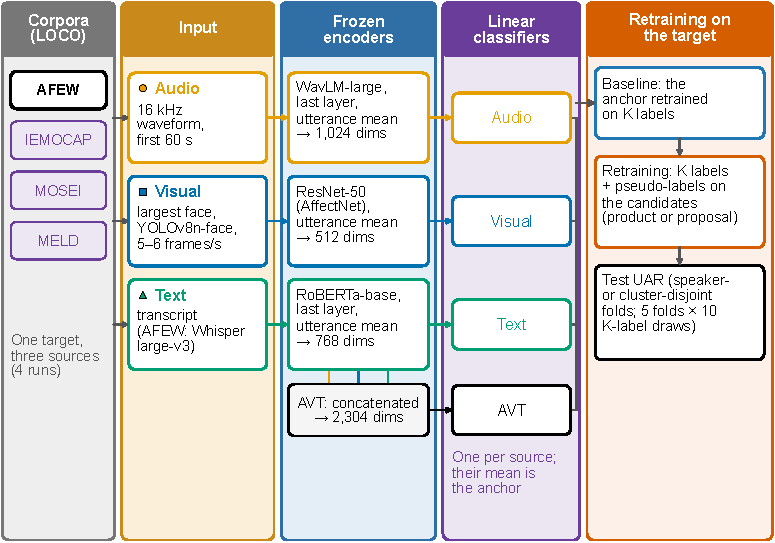
\includegraphics[width=\textwidth]{figures/fig_v4_pipeline_en.pdf}
\caption{Pipeline of the LOCO experiments. One of the four corpora is the target and the other three are the sources (four runs). The audio, visual and text inputs are passed through frozen encoders to give utterance-level features, and the three are also concatenated (AVT). Linear classifiers are trained per source, and the mean of the weights and intercepts of the three source classifiers is the anchor. On the target, the baseline (the anchor retrained on K labels per emotion) and classifiers retrained on the K labels and pseudo-labels on the candidate utterances (the product for the audio, visual, text and AVT classifiers; the proposal for the AVT classifier) are compared on the UAR of test utterances from speaker- or cluster-disjoint folds. AFEW is shown as the target. The evaluation of the proposal with CREMA-D as the target (Sects.~\ref{sec:res-prop}--\ref{sec:res-retrain} and Supplementary Information S7) uses audio and visual only, with four source corpora}\label{fig:pipeline}
\end{figure}

\subsection{Distillation and compared methods}\label{sec:distill}
Distillation retrains each of the audio, visual and text classifiers and the AVT classifier on pseudo-labels. The pseudo-label $q_i$ of each candidate utterance is the \emph{product}: the audio, visual and text classifiers are retrained from the anchor on the K labels and on the probabilities that the baseline AVT classifier assigns to the candidates, and their three probabilities are multiplied per utterance and normalised. $q_i$ includes the prediction of the retrained classifier's own modality. The loss of the retrained linear classifier is the cross-entropy on the K labels plus the cross-entropy towards the pseudo-labels of the candidates (the pseudo-label probabilities are targets without temperature) plus L2 terms towards the anchor $(W_0,b_0)$:
\begin{equation}
\begin{split}
L(W,b)=\frac{1}{S}\Big[&a\sum_{i\in\mathcal{K}}-\log p(y_i\mid x_i)+\sum_{i\in\mathcal{U}}\sum_k g_{ik}\,(-\log p(k\mid x_i))\\
&+\frac{\|W-W_0\|^2}{2C'}+\frac{\|b-b_0\|^2}{2C_b}\Big],
\end{split}
\end{equation}
with $p(\cdot\mid x)=\mathrm{softmax}(Wx+b)$ and $g_{ik}=(\rho n/4)\,q_{ik}/\sum_{j\in\mathcal{U}}q_{jk}$, where $\mathcal{K}$ is the set of K labelled utterances, $\mathcal{U}$ is the set of all $n$ candidates (including $\mathcal{K}$) and $S$ is the sum of the loss weights. The pseudo-label weights sum to $\rho n/4$ for each emotion. This loss form was fixed before the evaluation run; five other loss forms, including the temperature loss of Albanie et al.\ \cite{hinton2015distilling,albanie2018}, are compared in Supplementary Information S4. $C'$ and $C_b$ are those of the baseline; the pseudo-label weight $\rho$, the K-label multiplier $a$ and the exponents of each modality in the product were chosen on the mean UAR over provisional targets (Sect.~\ref{sec:protocol}); when several points were within two standard errors of the best, the one closest to the untuned values ($\rho=1$, $a=1$, exponents (1, 1, 1)) was chosen (grids in Supplementary Information S4). In all 48 conditions with K = 5, 10 and 25, the selected values gave the same classifier as the untuned values, so the product of distillation multiplies the three probabilities with equal weights.

In the LOCO setting, distillation is compared with 11 methods that do not use pseudo-labels including other modalities: self-training \cite{lee2013pseudolabel}, entropy minimisation \cite{grandvalet2004}, IM \cite{liang2020,boudiaf2020}, T3A \cite{iwasawa2021}, label propagation \cite{zhou2004,iscen2019}, a version that uses the retrained classifier's own baseline probabilities as pseudo-labels, training on labelled source utterances and the K labels together (S+T), CORAL \cite{sun2016coral}, DANN \cite{ganin2016dann}, MME \cite{saito2019mme} and an xMUDA-style method \cite{jaritz2020xmuda} (K = 5 UARs in Table~S4; content of each method in the notes of Table~S9). The xMUDA-style method makes unimodal classifiers imitate each other's predictions, so it uses predictions of other modalities but no pseudo-labels including other modalities (computed for the audio, visual and text classifiers only). All methods start from the same anchor and K labels as distillation and select hyperparameters by the same procedure. Because the encoders are frozen, DANN and MME are versions with their loss terms on a linear map and classifier, not the original methods that also train the feature extractor. In the all-source setting, the provider and weighting of the pseudo-labels of distillation were chosen per condition on provisional targets (mostly the product of the classifiers' probabilities), and distillation was compared with eight methods that use same-modality unlabelled utterances (entropy minimisation, self-training, IM, T3A, label propagation, CORAL, DANN and MME). The comparators of the combinations of predictions (Sects.~\ref{sec:res-prop} and \ref{sec:res-ablation}) and of the retrained AVT (Sect.~\ref{sec:res-retrain}) are described in those sections.

\textbf{Retraining with other pseudo-label providers.} In the evaluation run, each of the four classifiers was also retrained on predictions of other classifiers instead of the product, with untuned $\rho=1$ and $a=1$. The providers are classifiers of the baseline (unimodal classifiers of other modalities, classifiers on two concatenated modalities, AVT), the product, the three classifiers that make the product, the AVT anchor and the classifiers of each source corpus. K is 5 and 25, for which the candidate decisions of the baseline were saved. Excluding AVT retrained on its own predictions and duplicates of other providers leaves 360 variants per K (the excluded variants are in Supplementary Information S2; one of them, whose advantage is zero by construction, had a gain interval above zero). For each variant we measure (Fig.~\ref{fig:margintoy}):
\begin{itemize}
\item the \emph{advantage} (the difference in correctness of the pseudo-labels): UAR of the provider's decisions $-$ UAR of the baseline before retraining, on candidates excluding the K labels, using candidate labels that are never used for retraining;
\item the \emph{gain}: UAR of the retrained classifier $-$ UAR of the baseline on test utterances.
\end{itemize}


\begin{figure}[t]
\centering
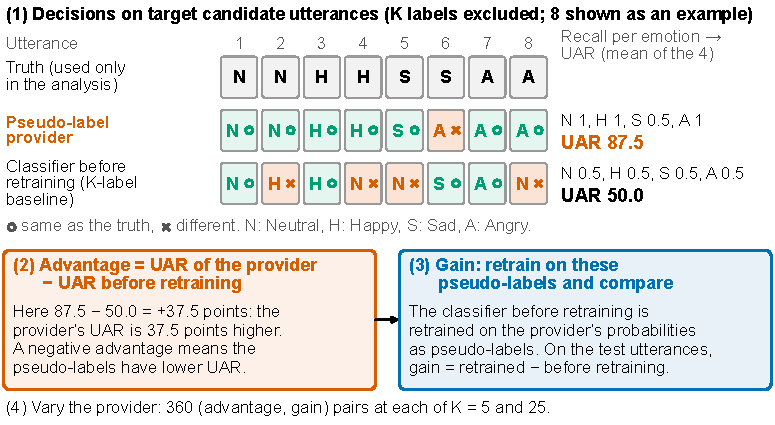
\includegraphics[width=\textwidth]{figures/fig_margin_toy_en.pdf}
\caption{Measuring the advantage and the gain. (1) On the candidate utterances excluding the K labels, the decisions of the pseudo-label provider and those of the classifier before retraining are each scored against the true labels, which are used only for this analysis, giving two UARs. (2) The advantage is the provider's UAR minus the UAR before retraining. (3) The classifier is retrained on the provider's probabilities as pseudo-labels, and the gain is measured on test utterances. (4) Repeating (2) and (3) for each provider gives the (advantage, gain) pairs. The eight utterances and their decisions are illustrative, not experimental values}\label{fig:margintoy}
\end{figure}

\subsection{Measuring the error that remains after removing bias}\label{sec:twoerrors}
A linear classifier assigns an emotion using, for each pair of emotions, a boundary in feature space whose direction is set by the weights and whose position is set by the intercepts (Fig.~S2). An error in which the boundary has the right direction but is shifted, so that predictions are biased towards one emotion, is the \emph{prediction bias}; it disappears when only the intercepts are corrected. The error that remains after correcting the bias is the \emph{remaining error}; it shrinks only when the direction of the weights changes.

We measure the remaining error, for each pair of emotions, as the pairwise accuracy lost because of the boundary direction (the \emph{direction loss}), computed from the distribution of decision values of test utterances relative to the linear discriminant direction of the labelled target utterances (formulas and the fit of the approximation in Supplementary Information S2). Changing only the intercepts, or subtracting each corpus's feature mean, does not change the direction loss. In the all-source setting, we measure whether distillation and each of the eight methods reduce the direction loss, averaged over the six emotion pairs, relative to the baseline. Each condition was classified by pre-set rules as \emph{reduced}, \emph{same level}, \emph{increased} or \emph{undetermined} from the 95\% interval of the direction-loss difference (baseline $-$ method) and an equivalence margin $\delta$ set from provisional-target outputs only (full rules, values of $\delta$ and intervals in Supplementary Information S2). Distillation is measured in 81 conditions (each classifier with audio, visual and text on three corpora and with audio and visual on five corpora; K = 0, 5, 25) and the eight methods in 210 conditions (single modality; K = 0, 5), so the two counts do not compare the same conditions.

\subsection{Proposal: pseudo-labels from per-emotion modality weights}\label{sec:method}

\subsubsection{Idea}\label{sec:idea}
Because distillation retrains classifiers towards pseudo-labels, the goal of the proposal is to raise the UAR of the pseudo-labels' decisions. The product of distillation multiplies the three classifiers' probabilities with equal weights. In computations run to design the method without the evaluation targets (the provisional-target runs of Sect.~\ref{sec:protocol}; each of the four corpora as a provisional target with two of the remaining corpora as sources, 30 repetitions each), the classifier-by-emotion reliabilities (Eq.~\ref{eq:rel} below) measured with all candidate labels were highest for visual on all four emotions of AFEW and for text on all four of MELD, for visual on Happy and audio on the others in IEMOCAP, and changed with the emotion in MOSEI (Fig.~\ref{fig:idea}). We therefore use 12 weights, one per classifier and emotion.

\begin{figure}[t]
\centering
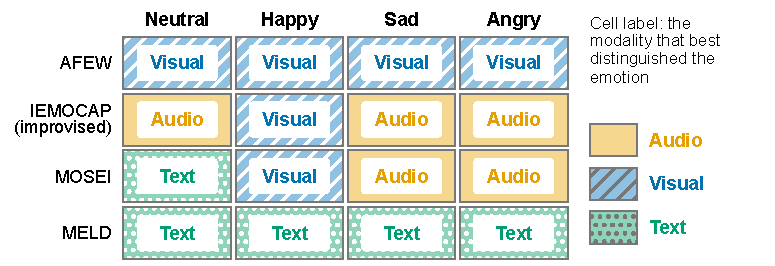
\includegraphics[width=\textwidth]{figures/fig_prop_idea_en.pdf}
\caption{The modality that best separated an emotion differed by corpus and by emotion. Each cell shows the modality with the highest reliability. Values are reliabilities used to design the method (provisional-target computations, all candidate labels, K = 5, mean of 30 repetitions), not values of the evaluation run}\label{fig:idea}
\end{figure}

Measuring all 12 weights on the K target labels would determine each weight from only K utterances per emotion. In the same provisional-target computations, we built two classifier-by-emotion reliability tables, one measured on the sources and one on all candidate labels of the provisional target, and found that splitting the weights into two parts allows each part to be measured on different data (values in Supplementary Information S5). The ranking of classifier strengths (mean reliability over the four emotions) changed across corpora. For every corpus and K, the strongest modality by source-measured strength differed from that on all candidate labels in more than half of the repetitions, and the K-label strengths agreed in more repetitions than the source-measured ones in 11 of the 12 combinations of corpus and K. The classifier-by-emotion component left after removing classifier effects, emotion effects and a non-additivity term, by contrast, correlated positively between the source table and the candidate-label table. We therefore measure strengths on the K target labels and per-emotion profiles on the labelled source corpora. Our goal is not to build a new fusion architecture that learns per-utterance weights, but to set weights that raise the UAR of the pseudo-labels while fitting only three quantities (one strength per classifier) on the K labels.

\subsubsection{Definition}\label{sec:method-def}
The proposal weights the predictions of the classifiers that make the product of distillation (Sect.~\ref{sec:distill}; the product components) with a classifier-by-emotion reliability table and turns the fused predictions into pseudo-labels. The table is the sum of strengths and per-emotion profiles (Fig.~S5). Figure~\ref{fig:propflow} shows how the proposal gives one unlabelled utterance its pseudo-label.

\begin{figure}[t]
\centering
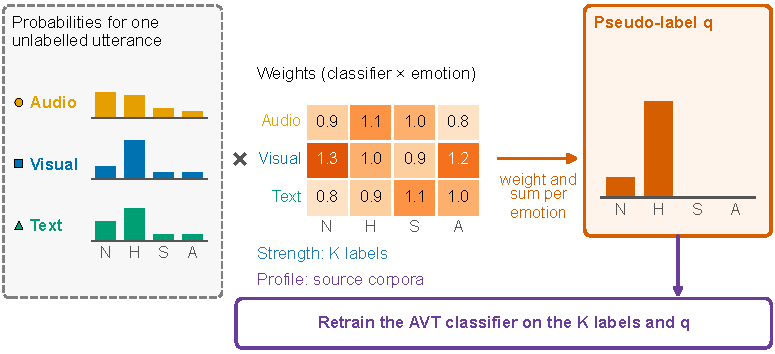
\includegraphics[width=\textwidth]{figures/fig_v4_prop_flow_en.pdf}
\caption{The proposal turns each unlabelled utterance into a pseudo-label q by multiplying the scores (centred log-probabilities) of the three classifiers by classifier-by-emotion weights and summing them per emotion. Left: probabilities that the audio, visual and text classifiers of the product (Sect.~\ref{sec:distill}) assign to one utterance. Middle: the weight table, built from the strengths (measured with classifiers retrained on the K labels without one of five subsets) and the per-emotion profiles (measured on the source corpora) and divided by its mean. Right: q, the softmax of the weighted sum after an intercept shift that uses no labels. The AVT classifier is retrained from the anchor on the K labels and q. Every candidate outside the test set, including the K labelled ones, receives q; test utterances are used only to measure UAR. Probabilities and weights are illustrative; q was computed with the intercept shift set to 0}\label{fig:propflow}
\end{figure}

The reliability is defined on the scores of each classifier. With probabilities $p_m(i\mid x)$ of classifier $m$ for emotion $i$, the centred log-probability is the score $z_m(i\mid x)=\log p_m(i\mid x)-\frac14\sum_j\log p_m(j\mid x)$, and
\begin{equation}\label{eq:rel}
d_m(i)=\max\!\big(0,\sqrt2\,\Phi^{-1}(A_m(i))\big),\quad A_m(i)\in[0.02,0.98],
\end{equation}
where $A_m(i)$ is the mean over emotions $j\neq i$ of the area under the ROC curve (AUC) separating utterances of true emotion $i$ from those of $j$ by $z_m(i\mid\cdot)$, and $\Phi^{-1}$ is the standard normal quantile function ($d_m(i)\le 2.90$). Because the ranks of scores do not change when intercepts are shifted, $d_m(i)$ depends neither on the classifier's intercepts nor on the target's emotion proportions. The mean over the four emotions is the strength $L_m$, and $d_m(i)-L_m$ is the per-emotion profile.

The strengths are measured on the K labels. The K labels are split into five subsets per emotion; for each subset $f$, the product components are retrained by the procedure of distillation on the K labels without subset $f$ and assign probabilities to subset $f$; the reliabilities of Eq.~(\ref{eq:rel}) computed from the five subsets' probabilities are averaged over emotions to give $L^{K}_m$. Because $L^{K}_m$ is noisy for small K, a default strength $L^{0}_m$ (the mean of the three $L^{K}_m$ or the strength measured on the sources) is mixed in with weight $n_0$:
\begin{equation}
L_m=\frac{n\,L^{K}_m+n_0\,L^{0}_m}{n+n_0},\qquad n=4K.
\end{equation}

The profiles are measured on the source corpora. Within each source $s$, $d^{\mathrm{in}}_{s,m}(i)$ is measured by speaker-split five-fold cross-validation, and a classifier trained on all of $s$ is applied to another source $t$ to give $d^{\mathrm{out}}_{s\to t,m}(i)$. The share of modality $m$'s reliability that carries over to other corpora is $\eta_m=\sum_{s\to t}\sum_i d^{\mathrm{out}}_{s\to t,m}(i)/\sum_{s\to t}\sum_i d^{\mathrm{in}}_{s,m}(i)$ (clipped to $[0,1.5]$), and
\begin{equation}
d^{\mathrm{src}}_m(i)=\eta_m\frac{1}{|S|}\sum_s d^{\mathrm{in}}_{s,m}(i),\qquad r^{\mathrm{src}}_m(i)=d^{\mathrm{src}}_m(i)-\frac14\sum_j d^{\mathrm{src}}_m(j)
\end{equation}

The reliability table combines strengths and profiles, and the fused predictions give the pseudo-labels. The table is $T(m,i)=\max(0,L_m+\beta\,r^{\mathrm{src}}_m(i))$ ($\beta=1$ uses the profiles, $\beta=0$ does not); dividing by its mean gives weights $\Omega(m,i)=T(m,i)/(\frac{1}{12}\sum_{m',i'}T(m',i'))$, and the scores are summed per emotion, $s(i\mid x)=\sum_m \Omega(m,i)\,z_m(i\mid x)$. Because emotion-specific weights can shift predictions towards some emotions, intercepts $c$ are shifted without labels so that the mean of $\mathrm{softmax}(s(\cdot\mid x)+c)$ over candidates equals the mean of the product's probabilities (fixed-point iteration). The fused prediction is $\arg\max_i(s(i\mid x)+c_i)$. We attach $q(i\mid x)=\mathrm{softmax}_i(s(i\mid x)+c_i)$ to the candidates as pseudo-labels (soft labels) and retrain the AVT classifier (AV for CREMA-D) with the loss of distillation (Sect.~\ref{sec:distill}). Because the fused predictions carry information of all three modalities, the retrained classifier is AVT, which takes all three features; comparisons of the fused predictions do not depend on this choice. Audio, visual and text classifiers retrained on the proposal's pseudo-labels were not computed (Sect.~\ref{sec:limitations}). $\rho$ and $a$ are borrowed from the values chosen for the product's pseudo-labels.

\subsubsection{Hyperparameters}\label{sec:hp}
The hyperparameters of the proposal ($n_0\in\{0,20,80,\infty\}$, $\beta\in\{0,1\}$ and the two default strengths; 16 settings, 14 distinct) were selected, per evaluation target and K, by the highest mean UAR on the test folds of the provisional targets over three episodes in which each source corpus served in turn as a provisional target with the other two as sources (3 corpora $\times$ 5 folds $\times$ 2 seeds = 30 repetitions; Fig.~S6). No data of the evaluation target enter any episode. All selected settings had $\beta=1$, and $n_0$ was 0 in 8 of 12 conditions and 20 in the other four. The setting $n_0=\infty$, $\beta=0$ with the mean default strength gives the same decisions as the product. For CREMA-D, the hyperparameters ($n_0=0$, $\beta=1$) and $\rho$ and $a$ for the AV classifier were selected on the repetitions of a six-corpus provisional-target computation (the four corpora plus CREMA-D and RAVDESS) that do not involve CREMA-D.

\subsection{Evaluation protocol and intervals}\label{sec:protocol}
LOCO hyperparameters were selected on runs in which each of the three corpora other than the evaluation target served in turn as a provisional target (with the remaining two corpora as sources; 3 corpora $\times$ 5 folds $\times$ 2 seeds = 30 repetitions) and fixed, and the evaluation target was computed once with the fixed settings (the evaluation run). We call each provisional-target computation an \emph{episode}.

The main metric is UAR (unweighted average recall over emotions), whose chance level with four emotions is 25\%. Overall accuracy (weighted accuracy) is not reported because it depends on the share of Neutral, which differs across corpora. UAR and its differences are in percentage points, and the difference A $-$ B between two classifiers is called the \emph{gain}. All intervals are 95\% intervals without multiple-comparison correction; they reflect the sampling of test speakers (clusters for MOSEI and the LOCO setting) and of the K labels, not the choice of source corpora, training utterances, methods or hyperparameters. For the LOCO setting, the variance of a cluster jackknife (cluster resampling for MOSEI and CREMA-D) is added to the variance over K-label draws; because inference with few clusters is anti-conservative \cite{cameron2008}, jackknife $t$ intervals are used for corpora with fewer than 20 effective test clusters. Intervals of the all-source setting are described in Supplementary Information S2. Conditions of the same corpus that differ only in K share test utterances and nested K labels and are not independent. We write that UAR \emph{rose} or \emph{fell} only when the 95\% interval of the difference lies above or below zero, and write ``higher'' or ``lower'' for point estimates.

The order of the work was as follows. The loss form and the hyperparameter grids of distillation were fixed before the evaluation run. The authors inspected UARs and differences (without intervals) of distillation and the 11 methods during the evaluation run (AFEW, IEMOCAP) and before aggregation (four corpora); aggregation scripts and designs were fixed before the evaluation run and not changed afterwards. The idea of the proposal was conceived after seeing outputs of the evaluation run of distillation, its form was fixed after seeing the provisional-target runs, and its evaluation was computed once. CREMA-D was added to the evaluation after its values had been seen in the six-corpus provisional runs. Some pseudo-label options of the all-source setting (such as the product) were added after seeing results of an earlier version of the method on the same corpora. The analysis with other pseudo-label providers (Sect.~\ref{sec:res-margin}) and the comparison with the strongest single classifier (Sect.~\ref{sec:res-prop}) were descriptive analyses set up after the computation from saved outputs, without prior predictions; the former was set up after the gains and intervals of audio, visual and text classifiers retrained on some providers had been seen. Variants share candidates, test utterances and pseudo-label ingredients, so the rank correlations and counts of Sect.~\ref{sec:res-margin} are not tests.
